\documentclass[11pt]{scrartcl}
\usepackage[sexy]{{style_files/evan}}

\usepackage{{style_files/NMC}}
\usepackage{standalone}
\usepackage{import}

\usetikzlibrary{shapes.geometric}

\begin{document}
\title{NMC Problem Set \#16} % add # of pset
\date{Dec. 4, 2022} % add date
\maketitle

\section*{Welcome!}

This is a selection of interesting problems derived from curious thoughts, curated so you can nibble on them throughout the week! The point of this document is to introduce you to fun puzzles that require thinking. We recommend you try the ones that you find interesting! Feel free to work on them with others (even us teachers!). Harder problems are marked with chilies (\fullchili), in case you want to challenge yourself.
\newline\newline
Have fun! \textit{Note: New variants on these problems may be released throughout the week. Remember to check back once in a while!}
    
\section{Algebra}
\begin{enumerate}[label=\textbf{A\arabic*}.]
    \item \textbf{Back to Square One} \newline
    Let $f : \mathbb R \to \mathbb R$ be a real-valued function. Suppose that $f$ is \emph{monotone}: it is either non-increasing ($x \ge y$ implies $f(x) \ge f(y)$) or non-decreasing ($x \le y$ implies $f(x) \le f(y)$).
    
    \begin{enumerate}
        \item Suppose that $f(f(z))$ for some real $z$. Prove that $f(z) = z$.
        \item Suppose that
        \[ f^n(z) = \underbrace{f(f(\cdots f(}_{\text{$n$ $f$'s}}z)\cdots)) = z, \]
        for some real $z$ and positive integer $n$. Prove that $f(z) = z$.
    \end{enumerate}
    
    \newpage
    
    \item \textbf{Regular Polygons are Nice} \newline
    Suppose we have a regular polygon with $n$ sides, inscribed in the unit circle, with vertices $A_1, A_2, A_3, \dots, A_n$. Draw all of the diagonals connected to $A_1$ (to all other vertices) so that we have a figure similar to the following:
    
    \begin{figure}[h]
        \centering
        \includegraphics[width = 8cm]{weekly/week 16/Diagrams/regpoly.tex}
        \hspace{2em}
        \caption{Example Diagram with $n = 11$. The product of the lengths of these diagonals is $11$. Sorry but Tikz isn't playing nice with me wanting to stick labels onto these vertices...}
        \label{fig:despicable}
    \end{figure}
    
    \begin{enumerate}
        \item Prove that the product of the lengths of these diagonals is equal to $n$. As in,
        \[ A_1A_2 \cdot A_1A_3 \cdot A_1A_4 \cdot \dots \cdot A_1A_n = n \]
        Note that this includes the lengths of the two sides that $A$ is connected to.
        
        \item Now, suppose we pick a point $P$ on our unit circle. Show that
        \[ PA_1^4 + PA_2^4 + PA_3^4 + \dots + PA_n^4 \]
        is constant.
        
        \item (\fullchili) Prove that if $n$ is odd, then all of $A_1A_2, A_1A_3, A_1A_4, \dots, A_1A_n$ are of irrational length.
    \end{enumerate}
    
    % add smth about https://math.stackexchange.com/questions/4494053/a-simple-problem-on-regular-polygon-inscribed-in-a-unit-circle
    % https://math.stackexchange.com/questions/1696869/regular-polygon-inscribed-in-a-unit-circle
\end{enumerate}

\clearpage
\section{Combinatorics}
\begin{enumerate}[label=\textbf{C\arabic*}.]
    \item \textbf{Lance is Evil} \newline
    An evil villain has trapped $100$ mathematicians. He makes them play the following game: each mathematician is assigned a hat, and on the hat is an integer from $1$ and $100$, of which the assigned numbers are not necessarily unique. \newline
    Each mathematician is not allowed to look at their own hat, nor communicate with others, but they can see the hats of others. If at least person is able to guess the number on their own hat, everyone will be set free.\\
    Everyone is allowed to formulate a strategy beforehand. Can the mathematicians escape?
\end{enumerate}

\newpage
\section{Geometry}
\begin{enumerate}[label=\textbf{G\arabic*}.]
    \item (Calculus, \fullchili) \textbf{Loading Screen Mechanics} \newline
    Find the volume swiped by a cube when it is rotated around its longest diagonal.
    \begin{figure}[h]
        \centering
        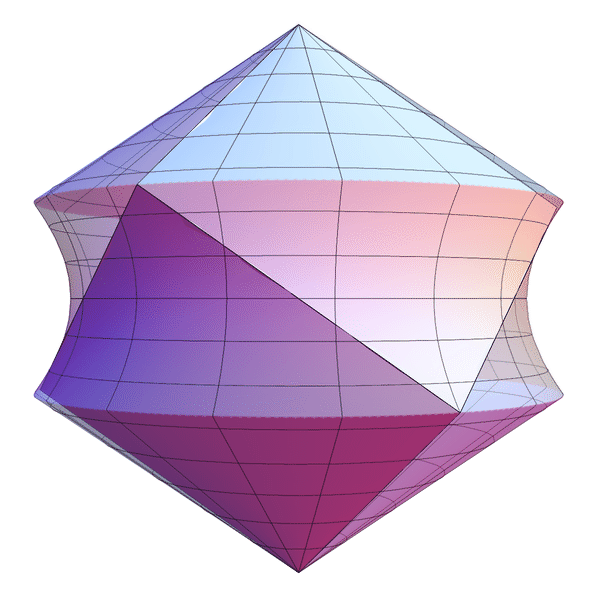
\includegraphics[width = 8cm]{weekly/week 16/Diagrams/revol.png}
        \hspace{2em}
        \label{fig:revol}
    \end{figure}
\end{enumerate}

\newpage
\section{Number Theory}
\begin{enumerate}[label=\textbf{N\arabic*}.]
    \item \textbf{Termination} \newline
    A sequence of primes $(p_n)$ satisfies $p_{n + 1} = 2p_n \pm 1$. Show that the sequence must be finite.
    
    \item \textbf{Prime Divisors} \footnote{LPD = London Police Department}
    \begin{enumerate}
        \item Find the smallest and largest prime divisors of $3^{15} + 1$.
        \item Find the smallest and largest prime divisors of $12^{2^{15}} + 1$.
    \end{enumerate}
\end{enumerate}

\end{document}
